% =============================================================================
%  Background for "The Mathematics of demo.py"
%  Build:  pdflatex beamformer_background.tex   (run twice for references / TOC)
%  Shares its preamble and glossary with beamformer_math.tex.
% =============================================================================
\documentclass[11pt]{article}
% =============================================================================
%  Shared preamble for beamformer_background.tex and beamformer_math.tex
%  (packages, colours, boxes, notation macros, glossary helpers)
% =============================================================================
\usepackage[margin=1in]{geometry}
\usepackage[T1]{fontenc}
\usepackage{lmodern}
\usepackage{microtype}
\usepackage{amsmath,amssymb,amsthm,mathtools,bm}
\usepackage{booktabs,array}
\usepackage{enumitem}
\usepackage{xcolor}
\usepackage{listings}
\usepackage{caption,subcaption}
\usepackage{placeins}
\usepackage{tikz}
\usetikzlibrary{arrows.meta,calc,positioning,decorations.pathreplacing,angles,quotes}
\usepackage{pgfplots}
\pgfplotsset{compat=1.18}
\usepgfplotslibrary{polar}
\usepackage[most]{tcolorbox}
\usepackage[colorlinks=true,linkcolor=blue!50!black,urlcolor=blue!50!black,citecolor=blue!50!black]{hyperref}

% ---------- theorem-like environments ----------------------------------------
\theoremstyle{plain}
\newtheorem{proposition}{Proposition}[section]
\theoremstyle{definition}
\newtheorem{definition}[proposition]{Definition}
\newtheorem{example}[proposition]{Worked example}
\theoremstyle{remark}
\newtheorem{remark}[proposition]{Remark}

% ---------- coloured boxes ---------------------------------------------------
\newtcolorbox{rationale}[1][]{breakable, enhanced, colback=orange!4, colframe=orange!60!black,
  boxrule=0.6pt, arc=2pt, left=6pt, right=6pt, top=4pt, bottom=4pt,
  title={Design rationale#1}, fonttitle=\bfseries\small, coltitle=black, colbacktitle=orange!15}
\newtcolorbox{intuition}{breakable, enhanced, colback=blue!3, colframe=blue!50!black,
  boxrule=0.6pt, arc=2pt, left=6pt, right=6pt, top=4pt, bottom=4pt,
  title={Intuition}, fonttitle=\bfseries\small, coltitle=black, colbacktitle=blue!10}
\newtcolorbox{inplainwords}{breakable, enhanced, colback=green!3, colframe=green!40!black,
  boxrule=0.6pt, arc=2pt, left=6pt, right=6pt, top=4pt, bottom=4pt,
  title={In plain words}, fonttitle=\bfseries\small, coltitle=black, colbacktitle=green!10}
\newtcolorbox{takeaways}{breakable, enhanced, colback=gray!4, colframe=gray!60!black,
  boxrule=0.6pt, arc=2pt, left=6pt, right=6pt, top=4pt, bottom=4pt,
  title={Key takeaways}, fonttitle=\bfseries\small, coltitle=black, colbacktitle=gray!15}
\newtcolorbox{checkyourself}{breakable, enhanced, colback=violet!3, colframe=violet!50!black,
  boxrule=0.6pt, arc=2pt, left=6pt, right=6pt, top=4pt, bottom=4pt,
  title={Check yourself}, fonttitle=\bfseries\small, coltitle=black, colbacktitle=violet!10}
\newtcolorbox{whereused}{enhanced, colback=white, colframe=gray!50,
  boxrule=0.4pt, arc=2pt, left=6pt, right=6pt, top=3pt, bottom=3pt, fontupper=\small}

% ---------- notation ---------------------------------------------------------
\newcommand{\herm}{^{\mathsf H}}
\newcommand{\tr}{^{\mathsf T}}
\newcommand{\vw}{\mathbf{w}}
\newcommand{\vd}{\mathbf{d}}
\newcommand{\vx}{\mathbf{X}}
\newcommand{\vn}{\mathbf{V}}
\newcommand{\vp}{\mathbf{p}}
\newcommand{\vu}{\mathbf{u}}
\newcommand{\one}{\mathbf{1}}
\newcommand{\mI}{\mathbf{I}}
\newcommand{\G}{\bm{\Gamma}}
\newcommand{\Gmu}{\bm{\Gamma}_{\!\mu}}
\newcommand{\E}{\mathbb{E}}
\newcommand{\code}[1]{\texttt{\detokenize{#1}}}
\newcommand{\WNG}{\mathrm{WNG}}
\newcommand{\DI}{\mathrm{DI}}

% ---------- glossary helpers -------------------------------------------------
% \term{key}{text}   : bold text in the body that links to the glossary entry `key`
% \gentry{key}{Name}{definition} : one glossary entry (used inside glossary.tex)
\newcommand{\term}[2]{\hyperlink{gls:#1}{\textbf{#2}}}
\newcommand{\gentry}[3]{\item[\hypertarget{gls:#1}{#2}] #3}

% ---------- code listings ----------------------------------------------------
\lstset{language=Python, basicstyle=\ttfamily\footnotesize, numbers=left,
  numberstyle=\tiny\color{gray}, numbersep=6pt, keywordstyle=\color{blue!70!black},
  commentstyle=\color{green!40!black}, stringstyle=\color{red!60!black},
  frame=single, rulecolor=\color{gray!50}, framexleftmargin=2pt, xleftmargin=12pt,
  breaklines=true, columns=fullflexible, keepspaces=true, showstringspaces=false}
\newcommand{\demolines}[2]{\lstinputlisting[firstline=#1,lastline=#2,firstnumber=#1]{demo.py}}

% ---------- figure styles ----------------------------------------------------
\tikzset{arr/.style={-{Stealth[length=2.2mm]}, thick}}
\definecolor{sdcol}{RGB}{200,70,30}
\definecolor{dascol}{RGB}{40,90,170}

\newcommand{\glsloc}[1]{}   % glossary section pointers only resolve in the main document

\title{\textbf{Background for \emph{The Mathematics of \texttt{demo.py}}}\\[4pt]
\large Sound, complex numbers, the FFT, and just enough linear algebra and probability}
\date{\today}

\begin{document}
\maketitle

\begin{abstract}
\noindent
The companion document, \emph{The Mathematics of \texttt{demo.py}} (\texttt{beamformer\_math.pdf}),
explains how seven tiny microphones can be combined into a directional ``acoustic zoom lens''.
That document assumes you are comfortable with waves, complex numbers, the Fourier transform and
complex-valued vectors. This one teaches those ideas from scratch. You only need Calculus~I
(derivatives, simple integrals, logarithms, $\sin$ and $\cos$) and an introductory linear algebra
course (vectors, matrices, dot products, solving $\mathbf A\mathbf x=\mathbf b$).

Every section ends with a \emph{Check yourself} question (answers in Section~\ref{sec:answers})
and a pointer to where the idea is used in the main document. Words in \textbf{bold blue} link to
the glossary at the end.
\end{abstract}

\tableofcontents

% =============================================================================
\section*{The big picture in one paragraph}
\addcontentsline{toc}{section}{The big picture in one paragraph}
% =============================================================================

Imagine seven people standing in a small circle, all listening to someone talking in front of
them. The sound reaches the person at the front of the circle a tiny bit earlier than the person
at the back. If each listener wrote down exactly what they heard, and we then \emph{slid} each
recording in time so that the talker's words lined up, adding the recordings would make the
talker's voice seven times stronger. Noise coming from other directions would \emph{not} line
up, so it would partly cancel. That is a \term{beamformer}{beamformer}. The rest of this
document builds the tools you need to describe that idea precisely: waves and delays
(Section~\ref{sec:waves}), digital samples (Section~\ref{sec:digital}), decibels
(Section~\ref{sec:db}), complex numbers, which turn delays into rotations
(Section~\ref{sec:complex}), the FFT, which splits sound into frequencies
(Section~\ref{sec:fft}), complex vectors and matrices (Section~\ref{sec:linalg}), noise
statistics (Section~\ref{sec:prob}) and constrained optimization (Section~\ref{sec:opt}).

\begin{table}[ht]
\centering\small
\begin{tabular}{@{}ll@{}}
\toprule
This document & Where the main document uses it\\
\midrule
\S\ref{sec:waves} Sound as a wave & \S2 Array geometry, \S3 Plane waves and the steering vector\\
\S\ref{sec:digital} Digital audio & \S7 Streaming, \S8 Gain staging\\
\S\ref{sec:db} Decibels & every plot and table; \S6 Beam pattern; \S8 Gain staging\\
\S\ref{sec:complex} Complex numbers and phasors & \S3 onward (the steering vector is made of phasors)\\
\S\ref{sec:fft} Frequency domain and the FFT & \S1 Overview, \S3, \S7 Streaming\\
\S\ref{sec:linalg} Complex vectors and matrices & \S4 Delay-and-sum, \S5 Superdirective\\
\S\ref{sec:prob} Noise, power and coherence & \S4 (array gain), \S5 (diffuse noise)\\
\S\ref{sec:opt} Optimization with a constraint & \S4 and \S5 (finding the best weights)\\
\bottomrule
\end{tabular}
\caption{Roadmap: which background section prepares you for which part of the main document.}
\end{table}
\FloatBarrier

% =============================================================================
\section{Sound as a wave}\label{sec:waves}
% =============================================================================

\subsection{Pressure, frequency and wavelength}

Sound is a tiny, rapid wiggle in air pressure that travels outward from its source. A microphone
measures that pressure at one point and turns it into a voltage. If a source hums a pure tone,
the pressure at a fixed point goes up and down like a sine wave:
\begin{equation}\label{eq:tone}
  p(t)=A\cos(2\pi f t+\theta).
\end{equation}
\begin{itemize}[nosep]
\item $A$ is the \term{amplitude}{amplitude}: how big the swings are.
\item $f$ is the \term{frequency}{frequency} in hertz (Hz): how many full cycles happen per second.
  The \emph{period} $T=1/f$ is the time one cycle takes.
\item $\theta$ is the \term{phase}{phase}: where in its cycle the wave is at $t=0$, measured as an
  angle. One full cycle is $360^\circ$, or $2\pi$ radians.
\end{itemize}
Real sounds such as speech are mixtures of many frequencies at once, roughly 100\,Hz to 8\,kHz for
speech. Section~\ref{sec:fft} shows how to separate them.

\begin{figure}[ht]
\centering
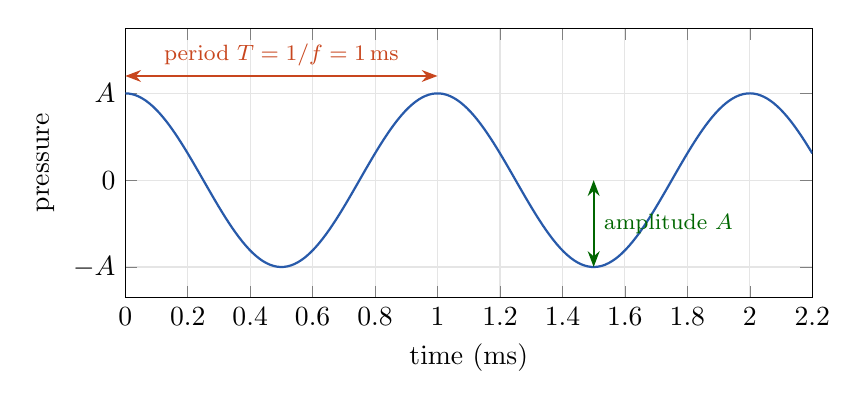
\begin{tikzpicture}
\begin{axis}[width=0.85\linewidth, height=5cm, xmin=0, xmax=2.2, ymin=-1.35, ymax=1.75,
  xlabel={time (ms)}, ylabel={pressure}, grid=major, grid style={gray!20}, samples=200,
  ytick={-1,0,1}, yticklabels={$-A$,$0$,$A$}]
  \addplot[thick, dascol, domain=0:2.2] {cos(deg(2*pi*x))};
  \draw[{Stealth[length=2mm]}-{Stealth[length=2mm]}, sdcol, thick] (axis cs:0,1.2) -- (axis cs:1,1.2)
    node[midway, above, font=\footnotesize] {period $T=1/f=1$\,ms};
  \draw[{Stealth[length=2mm]}-{Stealth[length=2mm]}, green!40!black, thick] (axis cs:1.5,0) -- (axis cs:1.5,-1)
    node[midway, right, font=\footnotesize] {amplitude $A$};
\end{axis}
\end{tikzpicture}
\caption{A 1\,kHz tone, $p(t)=A\cos(2\pi\cdot1000\,t)$, observed at one point in space.}
\label{fig:sine}
\end{figure}

Sound travels through air at about $c=343$\,m/s (at room temperature). In the time $T$ it takes
the source to complete one cycle, the wave moves forward a distance called the
\term{wavelength}{wavelength}:
\begin{equation}\label{eq:lambda}
  \lambda=cT=\frac{c}{f}.
\end{equation}

\begin{example}[How big are sound waves compared with our board?]\label{ex:lambda}
The UMA-8 microphone board is $86$\,mm across. Using $\lambda=343/f$:
\begin{center}\small
\begin{tabular}{@{}lccc@{}}
\toprule
frequency $f$ & 100\,Hz & 1\,kHz & 4\,kHz\\
\midrule
wavelength $\lambda$ & 3.43\,m & 34.3\,cm & 8.6\,cm\\
$\lambda$ compared with the board & 40$\times$ bigger & 4$\times$ bigger & about the same\\
\bottomrule
\end{tabular}
\end{center}
At low frequencies the wave is enormous compared with the array, so all seven mics hear almost
exactly the same thing. That makes low frequencies the hard case for a small array, and it is
the main reason the main document needs the ``superdirective'' design.
\end{example}

\subsection{Wavefronts, plane waves and time delays}

A \emph{wavefront} is a surface where the wave is at the same point in its cycle, for example
all the crests. Near a source the wavefronts are spheres. Far away, a small patch of a huge
sphere looks flat, so we model the sound as a \term{planewave}{plane wave}: flat, parallel
wavefronts marching in one direction. For an 86\,mm board, any talker more than about an arm's
length away is ``far'' (the \term{farfield}{far field}).

\begin{figure}[ht]
\centering
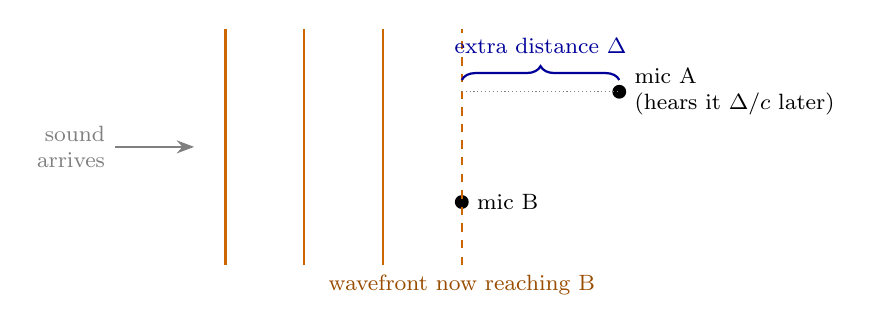
\begin{tikzpicture}[scale=1.0]
  % wavefronts are vertical lines; sound travels left -> right
  \foreach \x in {-2.4,-1.4,-0.4}{
    \draw[orange!80!black, thick] (\x,-1.5) -- (\x,1.5);}
  \draw[arr, gray] (-3.8,0) -- (-2.8,0) node[pos=0, left, font=\footnotesize, align=right] {sound\\arrives};
  \fill (0.6,-0.7) circle (2.5pt) node[right=2pt, font=\footnotesize] {mic B};
  \fill (2.6,0.7) circle (2.5pt) node[right=2pt, font=\footnotesize, align=left] {mic A\\(hears it $\Delta/c$ later)};
  \draw[orange!80!black, thick, dashed] (0.6,-1.5) -- (0.6,1.5);
  \node[font=\footnotesize, orange!60!black, below] at (0.6,-1.5) {wavefront now reaching B};
  \draw[densely dotted, gray] (0.6,0.7) -- (2.6,0.7);
  \draw[decorate, decoration={brace, amplitude=5pt}, blue!60!black, thick]
    (0.6,0.85) -- (2.6,0.85) node[midway, above=6pt, font=\footnotesize, align=center]
    {extra distance $\Delta$};
\end{tikzpicture}
\caption{A plane wave sweeps across two microphones. The one further ``downstream'' hears every
part of the sound later, by the extra distance divided by the speed of sound.}
\label{fig:planewave}
\end{figure}

The key fact for beamforming is simple:
\begin{equation}\label{eq:delay}
  \text{time difference}=\frac{\text{extra distance travelled}}{c}.
\end{equation}
The extra distance depends only on the \emph{direction} the sound comes from, so the set of
arrival-time differences across the array is a fingerprint of that direction. The main document
calls that fingerprint the \term{steering}{steering vector}.

\begin{example}[A real delay on the UMA-8]
Mic 5 on the UMA-8 sits $37.2$\,mm closer to the front than the centre mic. For a talker straight
ahead, it hears the sound $0.0372/343=108\,\mu$s (108 millionths of a second) earlier. That is
tiny. A 1\,kHz cycle lasts $1000\,\mu$s, so the head start is only about a tenth of a cycle.
\end{example}

\begin{checkyourself}
\begin{enumerate}[nosep]
\item What is the wavelength of a 2\,kHz tone in air?
\item The largest possible delay between the centre mic and a ring mic is $r/c$ with $r=43$\,mm.
  How many microseconds is that?
\end{enumerate}
\end{checkyourself}

\begin{whereused}
\textbf{Used in the main document:} \S2 (mic positions), \S3 (the plane-wave model and the delay
$\tau_m$), \S6 (why the array struggles at low and very high frequency).
\end{whereused}

% =============================================================================
\section{Digital audio}\label{sec:digital}
% =============================================================================

A computer cannot store a continuous curve, so it measures the microphone voltage at regular
instants. Each measurement is a \emph{sample}. The \term{samplerate}{sample rate} $f_s$ is the
number of samples per second, here $f_s=48\,000$, so consecutive samples are
$1/48\,000\approx20.8\,\mu$s apart. We write the $n$-th sample as $x[n]=x(n/f_s)$, using square
brackets for whole-number indices.

\begin{figure}[ht]
\centering
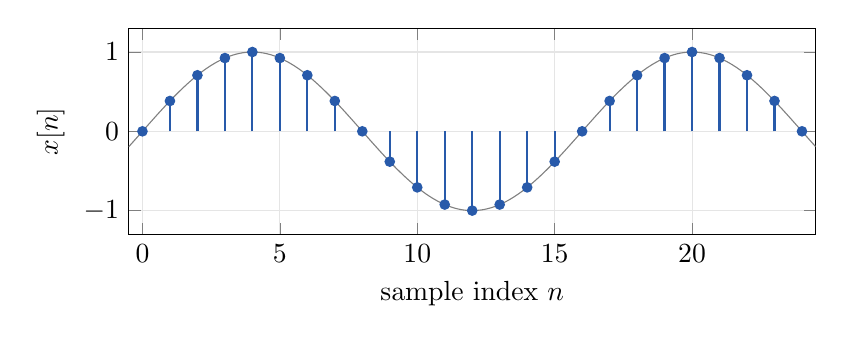
\begin{tikzpicture}
\begin{axis}[width=0.85\linewidth, height=4.2cm, xmin=-0.5, xmax=24.5, ymin=-1.3, ymax=1.3,
  xlabel={sample index $n$}, ylabel={$x[n]$}, grid=major, grid style={gray!20}, ytick={-1,0,1}]
  \addplot[gray, domain=-0.5:24.5, samples=200] {sin(deg(2*pi*x/16))};
  \addplot[ycomb, thick, dascol, mark=*, mark size=1.5pt, domain=0:24, samples=25] {sin(deg(2*pi*x/16))};
\end{axis}
\end{tikzpicture}
\caption{Sampling: the grey curve is the continuous signal, and the dots are the numbers the
computer actually stores (16 samples per cycle in this picture).}
\label{fig:samples}
\end{figure}

\paragraph{The Nyquist limit.} To capture a frequency you need at least two samples per cycle.
So the highest frequency a sampled signal can hold is the \term{nyquist}{Nyquist frequency}
$f_s/2$, which is 24\,kHz here and above the range of human hearing. A frequency above $f_s/2$ does
not vanish. It masquerades as a lower one, which is called \emph{aliasing}. The main document
meets a \emph{spatial} version of the same problem, where the ``samples'' are microphones spaced
in space instead of instants spaced in time.

\paragraph{Channels and blocks.} The UMA-8 delivers 8 \emph{channels} (7 mics and one spare),
each a stream of samples. The audio driver hands the program a \emph{block} of 256 new samples
per channel at a time, every $256/48\,000=5.33$\,ms. The program must return 256 output samples
before the next block arrives. This is why the main document cares so much about real-time
processing.

\paragraph{Full scale and clipping.} Here samples are floating-point numbers between $-1$ and $+1$.
The value $\pm1$ is \term{fullscale}{full scale}, the loudest the system can represent. Anything
bigger gets \term{clipping}{clipped}: flattened to $\pm1$, which sounds like harsh distortion.

\begin{checkyourself}
\begin{enumerate}[nosep]
\setcounter{enumi}{2}
\item The delay from question~2 is how many samples at 48\,kHz? Is it a whole number?
\end{enumerate}
\end{checkyourself}

\begin{whereused}
\textbf{Used in the main document:} \S1 (why fractional-sample delays push us to the frequency
domain), \S7 (blocks, hops, latency), \S8 (gain and clipping).
\end{whereused}

% =============================================================================
\section{Decibels}\label{sec:db}
% =============================================================================

Sound levels span a huge range: a whisper and a jet engine differ in pressure by a factor of about
a million. So engineers compare levels with a logarithmic unit, the
\term{db}{decibel} (dB). There are two versions, and they agree with each other because power is
proportional to amplitude squared:
\begin{equation}\label{eq:db}
  \text{amplitude ratio in dB}=20\log_{10}\frac{a_1}{a_2},\qquad
  \text{power ratio in dB}=10\log_{10}\frac{P_1}{P_2}.
\end{equation}

\begin{center}\small
\begin{tabular}{@{}lc@{\qquad}lc@{}}
\toprule
amplitude change & dB & power change & dB\\
\midrule
$\times1$ (unchanged) & $0$ & $\times1$ & $0$\\
$\times2$ & $+6.02$ & $\times2$ & $+3.01$\\
$\times\tfrac12$ & $-6.02$ & $\times\tfrac12$ & $-3.01$\\
$\times10$ & $+20$ & $\times10$ & $+10$\\
$\times16$ & $+24.08$ & $\times7$ & $+8.45$\\
\bottomrule
\end{tabular}
\end{center}

Three habits make dB easy:
\begin{itemize}[nosep]
\item \textbf{Multiplying ratios means adding dB.} A gain of 8 ($+18.06$\,dB) followed by a gain of
  2 ($+6.02$\,dB) is a gain of 16 ($+24.08$\,dB).
\item \textbf{0\,dB means ``no change''} and negative dB means ``smaller''. A beam pattern that reads
  $-20$\,dB at some angle passes sound from there at $1/10$ of its original amplitude.
\item \textbf{$-3$\,dB is the conventional ``edge''} of a beam: the angle where power has dropped to
  half.
\end{itemize}

\term{dbfs}{dBFS} means ``dB relative to full scale'': $0$\,dBFS is the loudest possible sample,
and real signals read negative values such as $-40$\,dBFS.

\begin{checkyourself}
\begin{enumerate}[nosep]
\setcounter{enumi}{3}
\item A beamformer reduces the noise \emph{power} by a factor of 7. How many dB is that?
\item The output gain is $8\times2^s$. How many dB does each extra step of $s$ add?
\end{enumerate}
\end{checkyourself}

\begin{whereused}
\textbf{Used in the main document:} every plot and table; white-noise gain and directivity index
(\S4--6); output gain and level meter (\S8).
\end{whereused}

% =============================================================================
\section{Complex numbers and phasors}\label{sec:complex}
% =============================================================================

This is the most important section. Complex numbers turn \emph{time delays} into
\emph{rotations}, and rotations are easy to add, undo and reason about.

\subsection{Complex numbers as arrows}

A \term{complex}{complex number} has the form $z=a+jb$, where $a$ and $b$ are ordinary real numbers
and $j$ is a symbol obeying $j^2=-1$. (Mathematicians write $i$. Engineers use $j$ because $i$ is
taken by electric current.) You add and multiply complex numbers like polynomials, replacing $j^2$
by $-1$:
\[
  (1+2j)+(3-j)=4+j,\qquad (1+2j)(3-j)=3-j+6j-2j^2=5+5j.
\]
Draw $z=a+jb$ as an arrow from the origin to the point $(a,b)$ in the \emph{complex plane}
(Figure~\ref{fig:complexplane}). Every arrow also has
\begin{itemize}[nosep]
\item a \textbf{magnitude} (length) $|z|=\sqrt{a^2+b^2}$, and
\item an \textbf{angle} (phase) $\theta$, measured counter-clockwise from the positive real axis.
\end{itemize}
The \term{conjugate}{conjugate} $\overline z=a-jb$ mirrors the arrow across the real axis, so it
has the same length and the opposite angle. A handy identity is $z\,\overline z=a^2+b^2=|z|^2$,
which is always real and never negative.

\begin{figure}[ht]
\centering
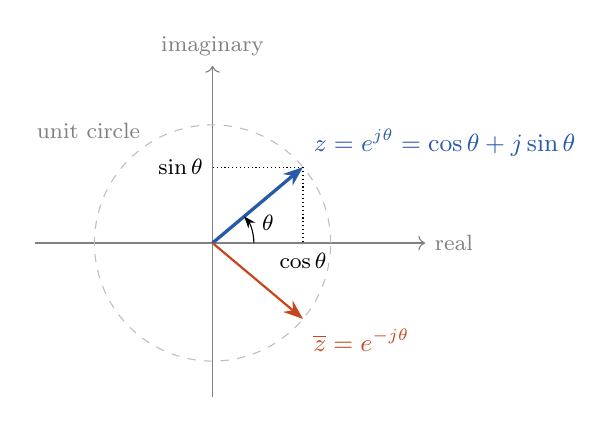
\begin{tikzpicture}[scale=1.5]
  \draw[->, gray] (-1.5,0) -- (1.8,0) node[right, font=\footnotesize] {real};
  \draw[->, gray] (0,-1.3) -- (0,1.5) node[above, font=\footnotesize] {imaginary};
  \draw[gray!50, dashed] (0,0) circle (1);
  \draw[-{Stealth[length=2.5mm]}, very thick, dascol] (0,0) -- (40:1)
    node[above right, font=\small] {$z=e^{j\theta}=\cos\theta+j\sin\theta$};
  \draw[-{Stealth[length=2.5mm]}, thick, sdcol] (0,0) -- (-40:1)
    node[below right, font=\small] {$\overline z=e^{-j\theta}$};
  \draw[densely dotted] (40:1) -- ({cos(40)},0) node[below, font=\footnotesize] {$\cos\theta$};
  \draw[densely dotted] (40:1) -- (0,{sin(40)}) node[left, font=\footnotesize] {$\sin\theta$};
  \draw[-{Stealth[length=1.5mm]}] (0.35,0) arc[start angle=0, end angle=40, radius=0.35];
  \node[font=\footnotesize] at (20:0.5) {$\theta$};
  \node[font=\footnotesize, gray] at (-1.05,0.95) {unit circle};
\end{tikzpicture}
\caption{The complex plane. A complex number of length~1 lies on the unit circle and is fully
described by its angle $\theta$. Its conjugate is its mirror image.}
\label{fig:complexplane}
\end{figure}

\subsection{Euler's formula: multiplying means rotating}

The single most useful formula in signal processing is \emph{Euler's formula}:
\begin{equation}\label{eq:euler}
  e^{j\theta}=\cos\theta+j\sin\theta.
\end{equation}
It says that $e^{j\theta}$ is the arrow of length~1 at angle $\theta$. (You can check it with the
Taylor series of $e^x$, $\cos x$ and $\sin x$ from calculus, but here we just use it.) Because
exponents add when you multiply,
\begin{equation}\label{eq:rotate}
  e^{j\alpha}\cdot e^{j\beta}=e^{j(\alpha+\beta)},
\end{equation}
multiplying by $e^{j\alpha}$ \emph{rotates} any arrow by angle $\alpha$ without changing its
length. Multiplying by the conjugate $e^{-j\alpha}$ rotates it back. Any complex number can be
written as $z=|z|\,e^{j\theta}$, a length times a direction.

\subsection{Phasors: a sinusoid is a spinning arrow}

Take the arrow $Ae^{j(2\pi ft+\theta)}$ and let time run. It spins around the origin $f$ times per
second, and its real part (the shadow on the real axis) is exactly the tone
$A\cos(2\pi ft+\theta)$ from \eqref{eq:tone}. All tones of the same frequency spin at the same
rate, so we can freeze the picture and keep only the starting arrow
\[
  \text{tone }A\cos(2\pi ft+\theta)\quad\longleftrightarrow\quad\text{\term{phasor}{phasor} }Ae^{j\theta}.
\]
The phasor's length is the amplitude and its angle is the phase. Adding two tones of the same
frequency is the same as adding their phasors as arrows.

\subsection{A time delay is a rotation}

Now combine this with Section~\ref{sec:waves}. If a microphone hears a tone $\tau$ seconds
\emph{later}, it records $A\cos(2\pi f(t-\tau)+\theta)=A\cos(2\pi ft+\theta-2\pi f\tau)$. The
phase has dropped by $2\pi f\tau$. In phasor language:
\begin{equation}\label{eq:delayrot}
  \boxed{\ \text{delay by }\tau\quad\Longleftrightarrow\quad\text{multiply the phasor by }e^{-j2\pi f\tau}\ }
\end{equation}
and hearing it $\tau$ seconds \emph{earlier} multiplies by $e^{+j2\pi f\tau}$. Notice that the
rotation angle $2\pi f\tau$ depends on frequency: the same time delay is a small rotation at low
frequency and a large one at high frequency.

\begin{example}[Mic 5 at 1\,kHz]
Mic 5 hears a talker straight ahead $\tau=108\,\mu$s early. At $f=1$\,kHz its phasor is
rotated by $2\pi f\tau=2\pi(1000)(0.000108)=0.68$\,rad $\approx39^\circ$ compared with the
centre mic. At 100\,Hz the same delay is only $3.9^\circ$.
\end{example}

\subsection{Adding phasors: reinforcement and cancellation}

This is the heart of beamforming. If seven phasors point the same way, their sum is seven times
longer. If they point in evenly spread directions, they cancel to zero
(Figure~\ref{fig:phasorsum}). A beamformer rotates each mic's phasor (by multiplying by a complex
\emph{weight}) so that sound from the chosen direction lines up and sound from other directions
does not.

\begin{figure}[ht]
\centering
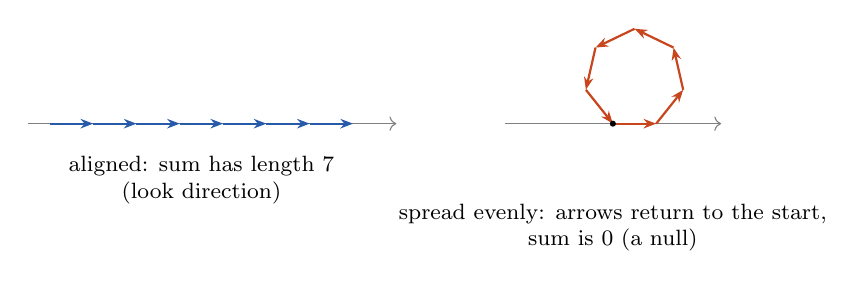
\begin{tikzpicture}[scale=0.55]
  \begin{scope}
    \draw[->, gray] (-0.5,0) -- (8,0);
    \foreach \i in {0,...,6}{\draw[-{Stealth[length=1.6mm]}, thick, dascol] (\i,0) -- (\i+1,0);}
    \node[font=\footnotesize, align=center] at (3.5,-1.3) {aligned: sum has length 7\\(look direction)};
  \end{scope}
  \begin{scope}[shift={(13,0)}]
    \draw[->, gray] (-2.5,0) -- (2.5,0);
    \coordinate (P) at (0,0);
    \foreach \i in {0,...,6}{
      \pgfmathsetmacro{\ang}{\i*360/7}
      \draw[-{Stealth[length=1.6mm]}, thick, sdcol] (P) -- ++(\ang:1) coordinate (P);
    }
    \fill (0,0) circle (2pt);
    \node[font=\footnotesize, align=center] at (0,-2.4) {spread evenly: arrows return to the start,\\sum is 0 (a null)};
  \end{scope}
\end{tikzpicture}
\caption{Adding seven unit phasors tip-to-tail. Left: in phase, they reinforce. Right: evenly
spread, they cancel completely.}
\label{fig:phasorsum}
\end{figure}

\begin{checkyourself}
\begin{enumerate}[nosep]
\setcounter{enumi}{5}
\item Compute $|3+4j|$ and $\overline{3+4j}$.
\item What is $e^{j\pi/2}$ in the form $a+jb$? What does multiplying by it do to an arrow?
\item A mic hears a 2\,kHz tone $125\,\mu$s late. By what angle (in degrees) is its phasor rotated,
  and in which direction?
\end{enumerate}
\end{checkyourself}

\begin{whereused}
\textbf{Used in the main document:} \S1 (``each delay becomes a phase rotation''), \S3 (the
steering vector is a list of phasors $e^{j2\pi f\tau_m}$), \S4 (delay-and-sum un-rotates them
with the conjugate).
\end{whereused}

% =============================================================================
\section{The frequency domain and the FFT}\label{sec:fft}
% =============================================================================

\subsection{Every sound is a sum of tones}

A remarkable fact, due to Fourier, is that \emph{any} reasonable signal can be written as a sum
of sinusoids of different frequencies, each with its own amplitude and phase. The list of those
amplitudes and phases (that is, a list of phasors, one per frequency) is the signal's
\emph{spectrum}. Looking at a signal this way is called working in the \emph{frequency domain}.

\begin{figure}[ht]
\centering
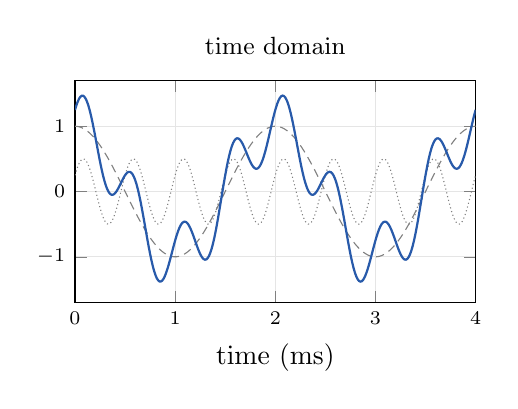
\begin{tikzpicture}
\begin{axis}[width=0.55\linewidth, height=4.4cm, xmin=0, xmax=4, ymin=-1.7, ymax=1.7,
  xlabel={time (ms)}, title={\small time domain}, samples=300, grid=major, grid style={gray!20},
  tick label style={font=\scriptsize}]
  \addplot[gray, densely dashed, domain=0:4] {cos(deg(2*pi*0.5*x))};
  \addplot[gray, densely dotted, domain=0:4] {0.5*cos(deg(2*pi*2*x)-60)};
  \addplot[thick, dascol, domain=0:4] {cos(deg(2*pi*0.5*x))+0.5*cos(deg(2*pi*2*x)-60)};
\end{axis}
\end{tikzpicture}\hfill
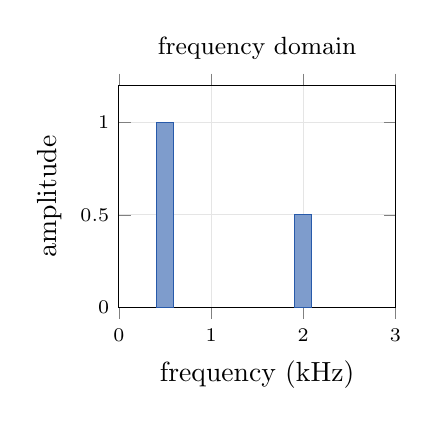
\begin{tikzpicture}
\begin{axis}[width=0.42\linewidth, height=4.4cm, xmin=0, xmax=3, ymin=0, ymax=1.2,
  xlabel={frequency (kHz)}, ylabel={amplitude}, title={\small frequency domain}, ybar,
  bar width=6pt, grid=major, grid style={gray!20}, tick label style={font=\scriptsize}]
  \addplot[fill=dascol!60, draw=dascol] coordinates {(0.5,1) (2,0.5)};
\end{axis}
\end{tikzpicture}
\caption{Left: the blue signal is the sum of a 500\,Hz tone (dashed) and a weaker 2\,kHz tone
(dotted). Right: its spectrum shows the same information as two bars. Each bar also carries a
phase, which this plot does not show.}
\label{fig:spectrum}
\end{figure}

\subsection{The DFT and FFT}

The \term{fft}{discrete Fourier transform} (DFT) does this for a block of $N$ samples
$x[0],\dots,x[N-1]$. It produces $N$ complex numbers
\begin{equation}\label{eq:dft}
  X[k]=\sum_{n=0}^{N-1}x[n]\,e^{-j2\pi kn/N},\qquad k=0,1,\dots,N-1.
\end{equation}
Read it as: ``for frequency number $k$, rotate each sample backwards by an amount that grows with
time, then add.'' If $x$ contains a tone at that frequency, the rotations cancel the tone's own
spinning, all the terms line up and the sum is large. Otherwise they spread out and mostly cancel,
exactly as in Figure~\ref{fig:phasorsum}. So $X[k]$ is the phasor (amplitude and phase) of the part
of the signal near frequency
\[
  f_k=k\,\frac{f_s}{N}.
\]
Each $k$ is called a \term{bin}{frequency bin}. The FFT (\emph{fast} Fourier transform) is just a
clever algorithm that computes the DFT in about $N\log_2N$ steps instead of $N^2$. The
\emph{inverse} FFT goes back from bins to samples, so no information is lost.

\begin{example}[The numbers in \texttt{demo.py}]
$N=512$ samples at $f_s=48$\,kHz gives bin spacing $48\,000/512=93.75$\,Hz. For a real-valued
signal the bins above $N/2$ are mirror images (conjugates) of the ones below, so NumPy's
\code{rfft} keeps only $k=0,\dots,256$: $257$ bins covering $0$ to $24$\,kHz.
\end{example}

\subsection{The shift theorem}

Section~\ref{sec:complex} showed that delaying a single tone rotates its phasor. Because every
signal is a sum of tones, the same holds bin by bin for any signal. This is the \emph{shift
theorem}:
\begin{equation}\label{eq:shift}
  x(t-\tau)\ \longrightarrow\ e^{-j2\pi f\tau}X(f),\qquad
  x(t+\tau)\ \longrightarrow\ e^{+j2\pi f\tau}X(f).
\end{equation}
This is why the main document works in the frequency domain. A delay of 2.3 samples is awkward to
apply to a list of samples, but in the frequency domain it is just a multiplication by a phasor,
one per bin.

\subsection{Frames, windows and the STFT}

Speech changes from moment to moment, so we cannot FFT the whole recording at once. Instead we
cut the signal into short overlapping \term{frame}{frames} (here 512 samples, $10.7$\,ms long,
each starting 256 samples after the previous one), multiply each frame by a smooth hill-shaped
\term{window}{window} that tapers its edges to zero, and FFT each frame. This is the
\term{stft}{short-time Fourier transform} (STFT). After processing, each frame is
inverse-FFT'd, windowed again and added back in place (\term{ola}{overlap-add}). With the right
window the overlapping pieces add up to exactly the original signal. The main document proves
this and explains the choice of window.

\begin{figure}[ht]
\centering
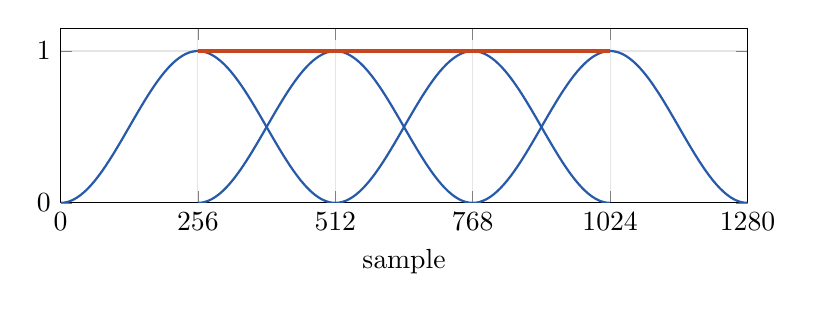
\begin{tikzpicture}
\begin{axis}[width=0.85\linewidth, height=3.8cm, xmin=0, xmax=2.5, ymin=0, ymax=1.15,
  xtick={0,0.5,...,2.5}, xticklabels={$0$,$256$,$512$,$768$,$1024$,$1280$}, ytick={0,1},
  xlabel={sample}, samples=80, grid=major, grid style={gray!20}]
  \foreach \s in {0,0.5,1,1.5}{
    \addplot[thick, dascol, domain=\s:\s+1] {sin(deg(pi*(x-\s)))^2};
  }
  \addplot[very thick, sdcol, domain=0.5:2] {1};
\end{axis}
\end{tikzpicture}
\caption{Overlapping frames, each weighted by a window (blue). Where two windows overlap they add
up to a constant (red), so nothing is lost or doubled.}
\label{fig:frames}
\end{figure}

\begin{checkyourself}
\begin{enumerate}[nosep]
\setcounter{enumi}{8}
\item With $f_s=48$\,kHz and $N=512$, which bin $k$ is closest to 1\,kHz, and what is its exact
  centre frequency?
\item In the frequency domain, what do you multiply bin $X(f)$ by to \emph{advance} the signal by
  $\tau$?
\end{enumerate}
\end{checkyourself}

\begin{whereused}
\textbf{Used in the main document:} \S1 (why frequency domain), \S3 (shift theorem
$\Rightarrow$ steering vector), \S7 (the full STFT and overlap-add machinery).
\end{whereused}

% =============================================================================
\section{Vectors and matrices with complex entries}\label{sec:linalg}
% =============================================================================

The main document handles all seven microphones at once by stacking their phasors into a vector.
Everything from your linear algebra course carries over, with one change: \emph{wherever you
transpose, also conjugate.}

\subsection{Vectors and the conjugate transpose}

At one frequency bin, the seven mic phasors form a column vector
$\mathbf x=[X_0,X_1,\dots,X_6]\tr$ in $\mathbb C^7$, the set of 7-entry complex vectors. The
\term{herm}{conjugate transpose} $\mathbf x\herm$ is the row vector of conjugated entries:
\[
  \mathbf x=\begin{bmatrix}1\\ j\end{bmatrix}
  \quad\Longrightarrow\quad
  \mathbf x\tr=\begin{bmatrix}1 & j\end{bmatrix},\qquad
  \mathbf x\herm=\begin{bmatrix}1 & -j\end{bmatrix}.
\]

\paragraph{Why conjugate?} The real dot product $\mathbf x\tr\mathbf x$ is a vector's squared length.
For complex vectors this breaks: the example above gives $\mathbf x\tr\mathbf x=1+j^2=0$, a
``length'' of zero for a nonzero vector. With the conjugate,
$\mathbf x\herm\mathbf x=1\cdot1+(-j)(j)=2$, which is correct. In general
\begin{equation}\label{eq:norm}
  \|\mathbf x\|^2=\mathbf x\herm\mathbf x=\sum_m|x_m|^2\ \ge 0.
\end{equation}

\paragraph{The complex dot product.} For two vectors,
$\mathbf w\herm\mathbf x=\sum_m\overline{w_m}\,x_m$. In the main document this \emph{is} the
beamformer: multiply each mic's phasor $x_m$ by a conjugated weight $\overline{w_m}$ (which
rotates and scales it) and add. If $w_m=e^{j\alpha_m}$, then $\overline{w_m}x_m$ rotates $x_m$
\emph{back} by $\alpha_m$, which is how delay-and-sum lines the phasors up.

\subsection{Matrices}

For a matrix $\mathbf A$, $\mathbf A\herm$ means transpose and conjugate every entry. A square
matrix with $\mathbf A\herm=\mathbf A$ is called \term{hermitian}{Hermitian}. It is the complex
version of a symmetric matrix, and its diagonal entries are always real. The identity matrix
$\mathbf I$ has ones on the diagonal and zeros elsewhere. Adding $\mu\mathbf I$ to a matrix adds
$\mu$ to every diagonal entry. The main document calls this ``\term{loading}{diagonal loading}''.

A Hermitian matrix is \emph{positive definite} if $\mathbf w\herm\mathbf A\mathbf w>0$ for every
nonzero $\mathbf w$. That quantity will be a noise power, so it should be positive. Positive
definite matrices are always invertible.

\subsection{Solving systems, and when that goes wrong}

To compute $\mathbf A^{-1}\mathbf b$, numerical code \emph{solves} $\mathbf A\mathbf x=\mathbf b$
(by elimination) instead of forming $\mathbf A^{-1}$ first. The result is the same, but solving
is faster and suffers less from rounding error. That is why \texttt{demo.py} calls
\code{np.linalg.solve}.

Some matrices are almost singular: their rows are nearly the same. Then a tiny change in
$\mathbf b$ makes a huge change in $\mathbf x$. The \term{cond}{condition number} measures how bad
this gets.

\begin{example}[An ill-conditioned $2\times2$ system]\label{ex:cond}
Let $\mathbf A=\begin{bmatrix}1&0.999\\0.999&1\end{bmatrix}$. This is what the noise coherence
between two mics looks like at low frequency, where the two mics hear almost identical noise.
\begin{itemize}[nosep]
\item With $\mathbf b=[1,\ 1]\tr$, the solution is $\mathbf x\approx[0.50,\ 0.50]\tr$.
\item Change $\mathbf b$ by just $1\%$, to $[1,\ 1.01]\tr$. The solution becomes
  $\mathbf x\approx[-4.5,\ 5.5]\tr$: large, with alternating signs.
\end{itemize}
This matrix's condition number is about 2000. The main document finds condition numbers up to
$10^{10}$ at 100\,Hz, and the cure, diagonal loading, works by making the diagonal a bit bigger
so the rows are less alike.
\end{example}

\begin{checkyourself}
\begin{enumerate}[nosep]
\setcounter{enumi}{10}
\item Let $\mathbf w=[1,\ j]\tr$ and $\mathbf x=[j,\ 1]\tr$. Compute $\mathbf w\herm\mathbf x$
  and $\|\mathbf w\|^2$.
\item Is $\begin{bmatrix}2 & j\\ -j & 2\end{bmatrix}$ Hermitian?
\end{enumerate}
\end{checkyourself}

\begin{whereused}
\textbf{Used in the main document:} \S3 (stacking mics into $\vx$ and $\vd$), \S4 (the
beamformer output $Y=\vw\herm\vx$), \S5 (solving with the coherence matrix, condition numbers,
diagonal loading).
\end{whereused}

% =============================================================================
\section{Noise, power and coherence}\label{sec:prob}
% =============================================================================

Noise is random, so we describe it by averages rather than exact values. Write $\E[\,\cdot\,]$
for the \emph{expected value}, the average over many repetitions (or, for steady noise, the
average over time).

\paragraph{Power.} The power of a zero-mean signal $v$ is its mean square, $\E[|v|^2]$. Its square
root is the RMS (root-mean-square) level that the \code{--levels} meter prints in dBFS. The
\term{snr}{signal-to-noise ratio} is
\[
  \text{SNR}=\frac{\text{signal power}}{\text{noise power}},\qquad\text{often in dB: }10\log_{10}\text{SNR}.
\]

\paragraph{Correlation and coherence.} For two noise signals $v_1,v_2$, the quantity
$\E[v_1\overline{v_2}]$ measures how much they move together. Dividing by their powers gives the
\term{coherence}{coherence}
\[
  \Gamma_{12}=\frac{\E[v_1\overline{v_2}]}{\sqrt{\E|v_1|^2\,\E|v_2|^2}},
\]
which is $1$ when the two signals are identical and $0$ when they are unrelated (independent).
For a whole array, these numbers fill a $7\times7$ \emph{coherence matrix}. Its diagonal is all
ones, because every mic is identical to itself. Like all such matrices, it is Hermitian.

Two kinds of noise matter in the main document:
\begin{itemize}[nosep]
\item \term{selfnoise}{Self-noise}: each mic's own electronic hiss. It is independent from mic to
  mic, so its coherence matrix is $\mathbf I$.
\item \term{diffuse}{Diffuse noise}: room echo and background chatter arriving from all
  directions. Mics that are close together compared with the wavelength hear nearly the same
  diffuse noise, so at low frequency its coherence is close to~1 for every pair.
\end{itemize}

\begin{example}[Why averaging $M$ mics helps against self-noise]\label{ex:avg}
Suppose each of $M$ mics records the same target $s$ plus its own independent noise $v_m$ of
power $\sigma^2$. Average them: $y=\frac1M\sum_m(s+v_m)=s+\frac1M\sum_m v_m$. The target is
unchanged. The noise power is
\[
  \E\Big|\tfrac1M\textstyle\sum_m v_m\Big|^2=\tfrac{1}{M^2}\displaystyle\sum_m\E|v_m|^2=\tfrac{1}{M^2}\cdot M\sigma^2=\tfrac{\sigma^2}{M},
\]
where the cross terms vanished because independent noises average to zero against each other.
So the SNR improves by a factor of $M$. With $M=7$, that is $10\log_{10}7=8.45$\,dB. The main
document calls this the \term{wng}{white-noise gain} of delay-and-sum, and proves it is the best
possible.

If the noise were \emph{identical} at every mic (coherence~1), averaging would not reduce it at
all. That is the low-frequency diffuse-noise problem the superdirective design attacks: instead
of adding, it cleverly \emph{subtracts} mics so the common noise cancels.
\end{example}

\begin{checkyourself}
\begin{enumerate}[nosep]
\setcounter{enumi}{12}
\item If you average 4 mics with independent noise, by how many dB does the SNR improve?
\item Two mics have noise coherence $0.99$. Will averaging them reduce that noise much? Why or
  why not?
\end{enumerate}
\end{checkyourself}

\begin{whereused}
\textbf{Used in the main document:} \S4 (signal model, noise covariance, array gain, WNG and DI),
\S5 (the diffuse-noise coherence matrix $\G$).
\end{whereused}

% =============================================================================
\section{Optimization with a constraint}\label{sec:opt}
% =============================================================================

Both beamformers in the main document come from the same kind of question:
\begin{quote}
\emph{Choose the weights $\mathbf w$ to make the output noise as small as possible, subject to the
rule that sound from the look direction passes through unchanged.}
\end{quote}
The rule is the \term{distortionless}{distortionless constraint} $\mathbf w\herm\mathbf d=1$.
Instead of Lagrange multipliers, the main document solves these problems with one inequality.

\subsection{The Cauchy--Schwarz inequality}

For real vectors you know $\mathbf a\cdot\mathbf b=\|\mathbf a\|\|\mathbf b\|\cos\theta$, where $\theta$
is the angle between them. Since $|\cos\theta|\le1$,
\begin{equation}\label{eq:cs}
  |\mathbf a\cdot\mathbf b|\le\|\mathbf a\|\,\|\mathbf b\|,
\end{equation}
with equality exactly when $\mathbf a$ and $\mathbf b$ point along the same line. This is the
\emph{Cauchy--Schwarz inequality}, and it holds for complex vectors too:
$|\mathbf a\herm\mathbf b|\le\|\mathbf a\|\,\|\mathbf b\|$, again with equality only when one
vector is a multiple of the other.

\subsection{A picture of the delay-and-sum solution}

Take the simplest case: minimise $\|\mathbf w\|^2$ (the self-noise power, by
Example~\ref{ex:avg}) subject to $\mathbf w\cdot\mathbf d=1$. In two real dimensions, the
constraint is a straight line, and we want the point on that line closest to the origin
(Figure~\ref{fig:cs}). Geometry says that point lies along $\mathbf d$, at
$\mathbf w=\mathbf d/\|\mathbf d\|^2$. Cauchy--Schwarz says the same thing algebraically:
$1=|\mathbf w\cdot\mathbf d|\le\|\mathbf w\|\|\mathbf d\|$, so $\|\mathbf w\|\ge1/\|\mathbf d\|$,
with equality only when $\mathbf w$ is parallel to $\mathbf d$.

\begin{figure}[ht]
\centering
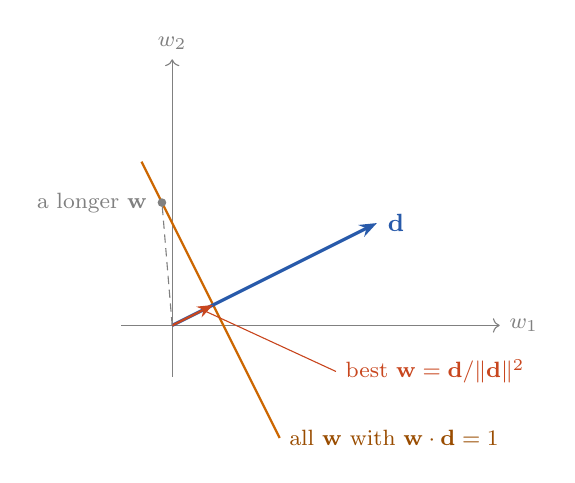
\begin{tikzpicture}[scale=1.3]
  \draw[->, gray] (-0.5,0) -- (3.2,0) node[right, font=\footnotesize] {$w_1$};
  \draw[->, gray] (0,-0.5) -- (0,2.6) node[above, font=\footnotesize] {$w_2$};
  % d = (2,1); constraint 2 w1 + w2 = 1  -> line through (0.5,0) and (0,1)
  \draw[thick, orange!80!black] (-0.3,1.6) -- (1.05,-1.1);
  \node[font=\footnotesize, orange!60!black, anchor=west] at (1.05,-1.1) {all $\mathbf w$ with $\mathbf w\cdot\mathbf d=1$};
  \draw[-{Stealth[length=2.2mm]}, very thick, dascol] (0,0) -- (2,1) node[right, font=\small] {$\mathbf d$};
  \draw[-{Stealth[length=2mm]}, thick, sdcol] (0,0) -- (0.4,0.2);
  \draw[sdcol, thin] (0.3,0.15) -- (1.6,-0.45);
  \node[sdcol, font=\footnotesize, anchor=west] at (1.6,-0.45) {best $\mathbf w=\mathbf d/\|\mathbf d\|^2$};
  \draw[densely dashed, gray] (0,0) -- (-0.1,1.2);
  \fill[gray] (-0.1,1.2) circle (1.2pt);
  \node[gray, font=\footnotesize, anchor=east] at (-0.15,1.2) {a longer $\mathbf w$};
\end{tikzpicture}
\caption{Minimising $\|\mathbf w\|$ on the constraint line. The shortest vector to the line is
perpendicular to it, which means parallel to $\mathbf d$. This is delay-and-sum in miniature.}
\label{fig:cs}
\end{figure}

The superdirective design in the main document is the same argument with the plain length
$\|\mathbf w\|^2$ replaced by a ``weighted length'' $\mathbf w\herm\G\mathbf w$ that measures
diffuse-noise power instead of self-noise power. The answer changes from
$\mathbf w\propto\mathbf d$ to $\mathbf w\propto\G^{-1}\mathbf d$, but the reasoning is identical.

\begin{checkyourself}
\begin{enumerate}[nosep]
\setcounter{enumi}{14}
\item In Figure~\ref{fig:cs}, $\mathbf d=[2,\ 1]\tr$. What is the best $\mathbf w$, and check that
  $\mathbf w\cdot\mathbf d=1$.
\item The steering vector has 7 entries, each of magnitude~1. What is $\|\mathbf d\|^2$, and what
  is the delay-and-sum weight $\mathbf w=\mathbf d/\|\mathbf d\|^2$?
\end{enumerate}
\end{checkyourself}

\begin{whereused}
\textbf{Used in the main document:} \S4 (Proposition: delay-and-sum is WNG-optimal), \S5
(Proposition: the MVDR/superdirective solution). Full proofs are in its Appendix~B.
\end{whereused}

\paragraph{You are ready.} If you can answer most of the ``Check yourself'' questions, you have every tool the
main document uses. Start with its Section~1, and use the glossary whenever a term is unclear.

% =============================================================================
\section{Answers to ``Check yourself''}\label{sec:answers}
% =============================================================================
\begin{enumerate}[leftmargin=2em]
\item $\lambda=343/2000=0.17$\,m $=17$\,cm.
\item $0.043/343=125\,\mu$s.
\item $125\,\mu\text{s}\times48\,000\text{/s}=6.0$ samples. That delay happens to be a whole number,
  but most delays in the array are not (for example $108\,\mu$s $=5.2$ samples). That is why the
  main document applies delays in the frequency domain.
\item $10\log_{10}7=8.45$\,dB (power ratio, so $10\log_{10}$).
\item $20\log_{10}2=6.02$\,dB.
\item $|3+4j|=\sqrt{9+16}=5$, and $\overline{3+4j}=3-4j$.
\item $e^{j\pi/2}=\cos90^\circ+j\sin90^\circ=j$. Multiplying by $j$ rotates an arrow by $90^\circ$
  counter-clockwise.
\item $2\pi f\tau=2\pi(2000)(0.000125)=\pi/2$ rad $=90^\circ$. A delay gives $e^{-j2\pi f\tau}$, so the
  rotation is clockwise (negative).
\item $1000/93.75=10.67$, so $k=11$ at $11\times93.75=1031.25$\,Hz. (This is why the main document's
  plots are labelled ``1031\,Hz''.)
\item $e^{+j2\pi f\tau}$.
\item $\mathbf w\herm\mathbf x=\overline{1}\cdot j+\overline{j}\cdot1=j-j=0$, and
  $\|\mathbf w\|^2=|1|^2+|j|^2=2$.
\item Yes. Transposing swaps the off-diagonal entries and conjugating flips their signs:
  $\overline{-j}=j$ and $\overline{j}=-j$, so you get the same matrix back.
\item $10\log_{10}4=6.02$\,dB.
\item No. The two noises are nearly identical, so they reinforce like the signal does and the
  averaging gains almost nothing. Subtracting them would cancel most of it.
\item $\|\mathbf d\|^2=5$, so $\mathbf w=[0.4,\ 0.2]\tr$, and $\mathbf w\cdot\mathbf d=0.8+0.2=1$.
\item $\|\mathbf d\|^2=7$, so $\mathbf w=\mathbf d/7$: each mic gets $1/7$ of the weight after its
  phase is lined up.
\end{enumerate}

% =============================================================================
\section{Glossary}\label{sec:glossary}
% =============================================================================
Plain-language definitions of the terms used in this document and in the main document.

% =============================================================================
%  Shared glossary.  \input by beamformer_background.tex and beamformer_math.tex.
%  Each document defines \glsloc{<label in beamformer_math>} itself:
%  the main document turns it into a section reference, the background
%  document ignores it.
% =============================================================================
\begin{description}[style=nextline, leftmargin=1.2em, itemsep=3pt, font=\normalfont\bfseries]

\gentry{aliasing}{Aliasing (spatial)}{When the microphones are too far apart compared with the
  wavelength, two different directions can produce the \emph{same} pattern of phases at the mics,
  so the array cannot tell them apart. For the UMA-8 this happens between front and back at about
  4.6\,kHz. It is the spatial version of sampling a signal too slowly in time.\glsloc{sec:aliasing}}

\gentry{amplitude}{Amplitude}{How big a wave's swings are, for example the peak pressure of a sound
  or the peak value of a digital sample. Doubling the amplitude adds about 6\,dB.}

\gentry{arraygain}{Array gain}{How much better the signal-to-noise ratio is at the beamformer output
  than at a single microphone, for a given kind of noise. White-noise gain and directivity index are
  two special cases.\glsloc{sec:das}}

\gentry{azimuth}{Azimuth ($\phi$)}{The horizontal direction a sound comes from, measured as an angle.
  In this project $\phi=0^\circ$ is the front of the board and positive angles are to the
  left.\glsloc{sec:geometry}}

\gentry{beampattern}{Beam pattern ($B$)}{A plot of how strongly the beamformer passes sound from
  each direction at a given frequency. It is $0$\,dB (unchanged) in the look direction and lower
  elsewhere. Its deep dips are called \emph{nulls}.\glsloc{sec:pattern}}

\gentry{beamformer}{Beamformer}{An algorithm that combines several microphone signals so that
  sound from one chosen direction is kept and sound from other directions is reduced: an
  ``acoustic zoom lens''.\glsloc{sec:overview}}

\gentry{bin}{Bin (frequency bin)}{One output of the FFT. Bin $k$ describes the part of the signal
  near frequency $f_k=k\,f_s/N$. Here the bins are $93.75$\,Hz apart and there are
  257 of them, from 0 to 24\,kHz.\glsloc{sec:steering}}

\gentry{circconv}{Circular convolution}{What filtering really does when you multiply FFT bins: the
  part of the filter's response that runs off the end of a frame wraps around to its start. It is
  usually small, and the window tapers hide most of it.\glsloc{sec:stft}}

\gentry{clipping}{Clipping}{Forcing any sample outside $[-1,1]$ back to $\pm1$. It causes brief
  distortion when the sound is too loud, but it prevents worse glitches.\glsloc{sec:gain}}

\gentry{coherence}{Coherence ($\Gamma_{ij}$)}{A number between $-1$ and $1$ saying how alike the noise
  at two microphones is: $1$ means identical, $0$ means unrelated. In diffuse noise, nearby mics at
  low frequency have coherence close to~1.\glsloc{sec:sd}}

\gentry{cola}{COLA (constant overlap-add)}{A property of a window: copies of it, shifted by the hop
  size and added together, sum to a constant. It guarantees that chopping a signal into frames and
  adding them back together returns the original signal.\glsloc{sec:stft}}

\gentry{complex}{Complex number}{A number $a+jb$ with a real part $a$ and an imaginary part $b$, where
  $j^2=-1$. Draw it as an arrow in a plane. It has a length (magnitude) and an angle (phase).
  Engineers write $j$ instead of $i$.}

\gentry{cond}{Condition number}{For a matrix, the factor by which a small error in the input can
  grow in the solution. A value near 1 is perfectly safe, and values like $10^{10}$ mean the answer
  is dominated by rounding errors and noise.\glsloc{sec:loading}}

\gentry{conjugate}{Conjugate ($\overline{z}$)}{Flip the sign of the imaginary part:
  $\overline{a+jb}=a-jb$. Geometrically, mirror the arrow across the real axis, which negates its
  angle. Multiplying by $\overline{e^{j\theta}}=e^{-j\theta}$ undoes a rotation by $\theta$.}

\gentry{herm}{Conjugate transpose ($\mathbf{A}\herm$)}{Transpose a vector or matrix (rows
  $\leftrightarrow$ columns) \emph{and} conjugate every entry. For vectors, $\vw\herm\vx$ is the
  complex version of the dot product. Also called the Hermitian transpose.}

\gentry{covariance}{Covariance matrix}{For a vector of random signals, the matrix of average products
  $\E[V_i\overline{V_j}]$. Its diagonal holds each signal's power and its off-diagonal entries show
  how related each pair is. Scaling it so the diagonal is~1 gives the coherence
  matrix.\glsloc{sec:das}}

\gentry{db}{Decibel (dB)}{A logarithmic way to compare two levels. For amplitudes use
  $20\log_{10}(a_1/a_2)$, and for powers use $10\log_{10}(P_1/P_2)$. $+6$\,dB is about twice the
  amplitude, $-3$\,dB is half the power, and $0$\,dB means ``unchanged''.}

\gentry{dbfs}{dBFS}{Decibels relative to \emph{full scale}, the loudest value the digital system can
  represent. $0$\,dBFS is the maximum, so every real signal reads negative.\glsloc{sec:gain}}

\gentry{das}{Delay-and-sum (DAS)}{The simplest beamformer. It undoes each mic's time head start so
  the target lines up, then averages. It is the best possible design against independent mic
  self-noise, but it is barely directional when the array is small compared with the
  wavelength.\glsloc{sec:das}}

\gentry{fft}{DFT / FFT}{The discrete Fourier transform turns a block of $N$ samples into $N$ complex
  numbers, one per frequency bin, each giving the amplitude and phase of that frequency. The FFT is
  a fast algorithm for computing it. \code{rfft} is the version for real-valued
  signals.\glsloc{sec:stft}}

\gentry{loading}{Diagonal loading ($\mu$)}{Adding a small number $\mu$ to every diagonal entry of the
  noise coherence matrix before designing the weights. It stops the design from amplifying mic
  self-noise too much. Here $\mu=0.05$.\glsloc{sec:loading}}

\gentry{diffuse}{Diffuse noise field}{Noise that arrives equally from every direction in 3-D, like
  room reverberation or a crowd of distant talkers. It is the noise the superdirective design is
  built to reject.\glsloc{sec:sd}}

\gentry{di}{Directivity index (DI)}{The array gain against diffuse noise, in dB: how much the beam
  favours its look direction over sound arriving from everywhere.\glsloc{sec:das}}

\gentry{distortionless}{Distortionless constraint}{The rule $\vw\herm\vd=1$. Sound from the look
  direction passes through every frequency bin with gain exactly~1, so the talker's voice is not
  coloured by the beamformer.\glsloc{sec:das}}

\gentry{farfield}{Far field}{Being far enough from the array that the arriving wavefronts are
  effectively flat. For this 86\,mm board, anything beyond about an arm's length
  qualifies.\glsloc{sec:steering}}

\gentry{frame}{Frame}{A short chunk of samples, here $N=512$ (10.7\,ms), that is windowed and
  sent through the FFT as one unit. Consecutive frames overlap by half.\glsloc{sec:stft}}

\gentry{frequency}{Frequency ($f$)}{How many times per second a wave repeats, in hertz (Hz). Human
  speech is mostly 100\,Hz--4\,kHz, and hearing extends to about 20\,kHz.}

\gentry{fullscale}{Full scale}{The largest value a digital audio sample can hold. In floating point
  this program uses $\pm1$.\glsloc{sec:gain}}

\gentry{hann}{Hann window}{A smooth hill-shaped window, $h[n]=\sin^2(\pi n/N)$, that tapers a frame to
  zero at both ends. Its square root is the sine window.\glsloc{sec:stft}}

\gentry{hermitian}{Hermitian matrix}{A square matrix equal to its own conjugate transpose,
  $\mathbf{A}=\mathbf{A}\herm$. It is the complex version of a symmetric matrix. Covariance and
  coherence matrices are always Hermitian.}

\gentry{hop}{Hop size ($H$)}{How many new samples arrive between one frame and the next, here 256.
  It equals the audio callback size.\glsloc{sec:stft}}

\gentry{latency}{Latency}{The delay between sound reaching the mics and coming out of the
  headphones. The algorithm adds $H/f_s=5.33$\,ms, and the sound device adds its own
  buffering.\glsloc{sec:stft}}

\gentry{leakage}{Spectral leakage}{The smearing of one frequency into neighbouring bins that happens
  when a frame is cut off abruptly. Tapering windows reduce it.\glsloc{sec:stft}}

\gentry{mems}{MEMS microphone}{A tiny microphone etched on a silicon chip (Micro-Electro-Mechanical
  System), like those in phones. The UMA-8 has seven of them.}

\gentry{mvdr}{MVDR}{Minimum-Variance Distortionless Response: choose the weights that make the
  output noise as small as possible while keeping the look direction exactly at gain~1. Applied to
  diffuse noise, it gives the superdirective beamformer.\glsloc{sec:sd}}

\gentry{nyquist}{Nyquist frequency}{Half the sample rate, $f_s/2$, which is 24\,kHz here. It is the
  highest frequency a sampled signal can represent without aliasing.}

\gentry{omni}{Omnidirectional}{Equally sensitive to sound from every direction. Each MEMS mic on its
  own is omnidirectional; only combining them makes a beam.}

\gentry{ola}{Overlap-add (OLA)}{Rebuilding a continuous output by adding the processed, overlapping
  frames back together at their original time positions.\glsloc{sec:stft}}

\gentry{phase}{Phase}{Where a wave is in its cycle, as an angle (one full cycle $=360^\circ=2\pi$
  radians). A time delay $\tau$ shifts a wave of frequency $f$ by phase
  $2\pi f\tau$.}

\gentry{phasor}{Phasor}{A complex number $Ae^{j\theta}$ that represents a sinusoid of a single
  frequency: its length is the amplitude and its angle is the phase. Adding sinusoids of the same
  frequency is the same as adding their arrows.}

\gentry{planewave}{Plane wave}{A wave whose wavefronts are flat parallel planes, which is a good
  model for sound from a distant source. All of its arrival-time differences come from the source
  direction alone.\glsloc{sec:steering}}

\gentry{samplerate}{Sample rate ($f_s$)}{How many samples per second a digital audio system takes,
  here 48\,000.}

\gentry{selfnoise}{Self-noise}{The faint hiss each microphone and its electronics produce on their
  own. It is independent from mic to mic, so it is ``white'' noise in the spatial
  sense.\glsloc{sec:das}}

\gentry{sinewin}{Sine window}{$g[n]=\sin(\pi n/N)$, the square root of the Hann window. This program
  applies it both before the FFT and after the inverse FFT.\glsloc{sec:stft}}

\gentry{snr}{SNR}{Signal-to-noise ratio: the power of what you want divided by the power of what you
  don't, usually given in dB.}

\gentry{steering}{Steering vector ($\vd$)}{The list of seven phase factors, one per mic, that a plane
  wave from a given direction at a given frequency produces. It is the array's ``fingerprint'' for
  that direction.\glsloc{sec:steering}}

\gentry{stft}{STFT}{Short-time Fourier transform: chop the signal into overlapping windowed frames and
  FFT each one, which shows how the frequency content changes over time.\glsloc{sec:stft}}

\gentry{superdirective}{Superdirective beamformer}{A beamformer designed to reject diffuse noise.
  It is far more directional than delay-and-sum on a small array at low frequency, at the cost of
  amplifying mic self-noise.\glsloc{sec:sd}}

\gentry{unitvector}{Unit vector}{A vector of length 1, used only to indicate a direction. Here $\vu$
  points from the array toward the source.\glsloc{sec:steering}}

\gentry{wavelength}{Wavelength ($\lambda$)}{The distance between neighbouring wave crests,
  $\lambda=c/f$. At 1\,kHz in air it is 34\,cm, four times the size of the board.}

\gentry{wavenumber}{Wavenumber ($\kappa$)}{$\kappa=2\pi f/c=2\pi/\lambda$: how many radians of phase a
  wave accumulates per metre travelled.\glsloc{sec:steering}}

\gentry{wng}{White-noise gain (WNG)}{The array gain against independent mic self-noise. It is
  $1/\|\vw\|^2$ for a distortionless beamformer. A negative WNG in dB means the beamformer makes the
  hiss \emph{louder} than a single mic would.\glsloc{sec:das}}

\gentry{window}{Window (function)}{A curve multiplied onto a frame to taper its edges smoothly toward
  zero, which avoids clicks and spectral leakage.\glsloc{sec:stft}}

\end{description}


\end{document}
